%%%%%%%%%%%%%%%%%%%%%%%%%%%%%%%%%%%%%%%%%%%%%%%%%%%%%%%%%%%%
%%  Class 1, NE 255
%%

\documentclass[xcolor=x11names,compress, handout]{beamer}

\definecolor{CoolBlack}{rgb}{0.0, 0.18, 0.39}
%% General document %%%%%%%%%%%%%%%%%%%%%%%%%%%%%%%%%%
\usepackage{graphicx}
\usepackage{tikz}
\usetikzlibrary{decorations.fractals}
\usepackage{hyperref}
%%%%%%%%%%%%%%%%%%%%%%%%%%%%%%%%%%%%%%%%%%%%%%%%%%%%%%

%% Beamer Layout %%%%%%%%%%%%%%%%%%%%%%%%%%%%%%%%%%
\useoutertheme[subsection=false,shadow]{miniframes}
\useinnertheme{default}
\usefonttheme{serif}
\usepackage{palatino}
\usepackage{tabu}
% Links
\usepackage{hyperref}
\definecolor{links}{HTML}{003262}
\hypersetup{colorlinks,linkcolor=,urlcolor=links}

% addition of color
\usepackage{xcolor}
\definecolor{CoolBlack}{rgb}{0.0, 0.18, 0.39}
\definecolor{byellow}{rgb}{0.55037, 0.38821, 0.06142}
\definecolor{dgreen}{rgb}{0.,0.6,0.}
\definecolor{RawSienna}{cmyk}{0,0.72,1,0.45}
\definecolor{forestgreen(web)}{rgb}{0.13, 0.55, 0.13}
\definecolor{cardinal}{rgb}{0.77, 0.12, 0.23}

\setbeamerfont{title like}{shape=\scshape}
\setbeamerfont{frametitle}{shape=\scshape}

\setbeamercolor*{lower separation line head}{bg=CoolBlack}
\setbeamercolor*{normal text}{fg=black,bg=white}
\setbeamercolor*{alerted text}{fg=dgreen} % just testing; I think this looks better
\setbeamercolor*{example text}{fg=black}
\setbeamercolor*{structure}{fg=black}

\setbeamercolor*{palette tertiary}{fg=black,bg=black!10}
\setbeamercolor*{palette quaternary}{fg=black,bg=black!10}

% Margins
\usepackage{changepage}

\mode<presentation>
{
  \definecolor{berkeleyblue}{HTML}{003262}
  \definecolor{berkeleygold}{HTML}{FDB515}
  \usetheme{Boadilla}      % or try Darmstadt, Madrid, Warsaw, Boadilla...
  %\usecolortheme{dove} % or try albatross, beaver, crane, ...
  \setbeamercolor{structure}{fg=berkeleyblue,bg=berkeleygold}
  \setbeamercolor{palette primary}{bg=berkeleyblue,fg=white} % changed this
  \setbeamercolor{palette secondary}{fg=berkeleyblue,bg=berkeleygold} % changed this
  \setbeamercolor{palette tertiary}{bg=berkeleyblue,fg=white} % changed this
  \usefonttheme{structurebold}  % or try serif, structurebold, ...
  \useinnertheme{circles}
  \setbeamertemplate{navigation symbols}{}
  \setbeamertemplate{caption}[numbered]
  \usebackgroundtemplate{}
}
%---

\renewcommand{\(}{\begin{columns}}
\renewcommand{\)}{\end{columns}}
\newcommand{\<}[1]{\begin{column}{#1}}
\renewcommand{\>}{\end{column}}

% adding slide numbers
\addtobeamertemplate{navigation symbols}{}{%
    \usebeamerfont{footline}%
    \usebeamercolor[fg]{footline}%
    \hspace{1em}%
    \insertframenumber/\inserttotalframenumber
}

% equation stuff
\newcommand{\Macro}{\ensuremath{\Sigma}}
\newcommand{\Sn}{\ensuremath{S_N} }
\newcommand{\vOmega}{\ensuremath{\hat{\Omega}}}
\usepackage{mathrsfs}
\usepackage[mathcal]{euscript}
\usepackage{amssymb}
\usepackage{amsthm}
\usepackage{epsfig}
\usepackage{amsmath}
%%%%%%%%%%%%%%%%%%%%%%%%%%%%%%%%%%%%%%%%%%%%%%%%%%
% title stuff for footer
\title{NE 255}
\author{R.\ N.\ Slaybaugh}
\date{August 25, 2016}

\begin{document}

%%%%%%%%%%%%%%%%%%%%%%%%%%%%%%%%%%%%%%%%%%%%%%%%%%%%%%
%%%%%%%%%%%%%%%%%%%%%%%%%%%%%%%%%%%%%%%%%%%%%%%%%%%%%%
\begin{frame}
\title{NE 255\\Numerical Simulations in Radiation Transport}
\subtitle{Lecture 1: Introduction}
\titlepage
\end{frame}

%%%%%%%%%%%%%%%%%%%%%%%%%%%%%%%%%%%%%%%%%%%%%%%%%%%%%%
%%%%%%%%%%%%%%%%%%%%%%%%%%%%%%%%%%%%%%%%%%%%%%%%%%%%%%
\begin{frame}{Details + Explanation}

Let's go over the syllabus!

\begin{itemize}
\item What this class is about: this is my first time teaching it, so there is a lot of space for adjustment.

\item Basic programming skills = you know \textit{some} language and can write a short program. Extra helpful if you can make functions/subroutines.

\item I give bonus points for
  \begin{itemize}
  \item submitting a pull request to correct course notes
  \item submitting your homework as a link to a Git repo (note: I still need to be able to figure out what on earth you did)
  \end{itemize}
If you don't know how to use Git...
\end{itemize}

\end{frame}

%%%%%%%%%%%%%%%%%%%%%%%%%%%%%%%%%%%%%%%%%%%%%%%%%%%%%%
%%%%%%%%%%%%%%%%%%%%%%%%%%%%%%%%%%%%%%%%%%%%%%%%%%%%%%
\begin{frame}{References \& Resources}

\begin{itemize}
\item The links in the syllabus are clickable; many are repeated in the helpful resources page.

\item There are a lot of books listed: 
  \begin{itemize}
  \item some are available electronically
  \item I have extra copies of Lewis \& Miller in my office for loan
  \item mostly you'll just use course notes 
  \end{itemize}

\item I haven't actually decided if we'll use MCNP. If you're interested in it for a final project (a) request access now, (b) you might want to request exe only, (c) I won't let you use MCNP for a final project unless you already have experience with it or you make a very compelling case. 
\end{itemize}

\end{frame}


%%%%%%%%%%%%%%%%%%%%%%%%%%%%%%%%%%%%%%%%%%%%%%%%%%%%%%
%%%%%%%%%%%%%%%%%%%%%%%%%%%%%%%%%%%%%%%%%%%%%%%%%%%%%%
\begin{frame}{DECF}

\begin{itemize}
\item Class time reserved 
  \begin{itemize}
  \item Tuesdays 4\textemdash 6 pm
  \item Fridays 1\textemdash 3 pm
  \end{itemize}

\item DECF Online Help: \href{http://www.decf.berkeley.edu/help/}{http://www.decf.berkeley.edu/help/}	

\item How to use SSH to access DECF computers: \href{http://www.decf.berkeley.edu/help/apps/ssh/}{http://www.decf.berkeley.edu/help/apps/ssh/}

\item Archipelagos Linux Cluster	
  \begin{itemize}
  \item Access is through SSH ONLY	
  \item 12 Linux nodes, 26 CPUs
  \end{itemize}

\item 1111 Linux Cluster		
  \begin{itemize}
  \item Access is through SSH ONLY
  \item 25 Linux nodes, 100 CPUs
  \end{itemize}

\item DECF Linux Clusters Status \href{http://www.decf.berkeley.edu/ganglia/}{http://www.decf.berkeley.edu/ganglia/}

\end{itemize}

\end{frame}


%%%%%%%%%%%%%%%%%%%%%%%%%%%%%%%%%%%%%%%%%%%%%%%%%%%%%%
%%%%%%%%%%%%%%%%%%%%%%%%%%%%%%%%%%%%%%%%%%%%%%%%%%%%%%
\begin{frame}{DECF cont'd}

\begin{itemize}
\item Main Server
  \begin{itemize}
  \item Kepler (kepler.berkeley.edu) 1.4 Mhz Dell Poweredge 1650 Linux server, 2 GB of real memory	
  \item Login server for DECF (DO NOT RUN JOBS ON KEPLER)	
  \end{itemize}

\item 1111 Etcheverry Lab	
  \begin{itemize}
  \item 11 Precision T3500 Workstations (Intel Xeon Quad Core, 6GB RAM)
  \item 13 Precision T3400 Workstations (Intel Core 2 Quad, 2GB RAM)	
  \item 2 HP 4350 black \& white laserjet printers
  \end{itemize}

\item The 1111 Linux Cluster (\textit{machinename.decf.berkeley.edu})	

\begin{tabular}{lllll}
boogie& bump& chacha& charleston& fandango\\
fever& flamenco& foxtrot & freeze& jitterbug\\
jive& lindy-hop& macarena& mambo & mazurka\\
merengue& minuet & polka& quickstep& rumba\\
salsa& sidekick& sock-hop& stomp&
\end{tabular}

\end{itemize}

\end{frame}


%%%%%%%%%%%%%%%%%%%%%%%%%%%%%%%%%%%%%%%%%%%%%%%%%%%%%%
%%%%%%%%%%%%%%%%%%%%%%%%%%%%%%%%%%%%%%%%%%%%%%%%%%%%%%
\begin{frame}{Savio}

\begin{itemize}
\item BRC manages SAVIO, the new high-performance computational
cluster for research computing.	

\item Unlike traditional clusters, SAVIO is a collaborative system
wherein the majority of nodes are purchased and shared by the cluster users, known as condo owners: \href{http://research-it.berkeley.edu/services/high-performance-
computing/institutional-and-condo-computing}{http://research-it.berkeley.edu/services/high-performance-
computing/institutional-and-condo-computing}		

\item Several types of hardware are available: \href{http://research-it.berkeley.edu/services/high-performance-computing/user-guide\#Hardware}{http://research-it.berkeley.edu/services/high-performance-computing/user-guide\#Hardware}	
\end{itemize}

\end{frame}


%%%%%%%%%%%%%%%%%%%%%%%%%%%%%%%%%%%%%%%%%%%%%%%%%%%%%%
%%%%%%%%%%%%%%%%%%%%%%%%%%%%%%%%%%%%%%%%%%%%%%%%%%%%%%
\begin{frame}{Campus Info + Integrity}

\textbf{Useful Campus Information:} 
\begin{itemize}
  \item Mental health resources: \href{http://www.uhs.berkeley.edu/students/counseling/cps.shtml}{http://www.uhs.berkeley.edu/students/counseling/cps.shtml}
  \item Sexual assault support on campus: \href{http://survivorsupport.berkeley.edu/}{http://survivorsupport.berkeley.edu/}
  \item Berkeley’s honor code is ``As a member of the UC Berkeley community, I act with honesty, integrity, and respect for others."
\end{itemize}

\vspace*{1 em}
I pledge to honor my word and act with respect towards you as a class. \\
I request you endeavor to do the same.\\ 
Everything can be worked out in communication. 

\end{frame}

%%%%%%%%%%%%%%%%%%%%%%%%%%%%%%%%%%%%%%%%%%%%%%%%%%%%%%
%%%%%%%%%%%%%%%%%%%%%%%%%%%%%%%%%%%%%%%%%%%%%%%%%%%%%%
\begin{frame}{Topics and Schedule}
\begin{itemize}
\item The list of topics from previous versions of this course has some overlap with NE155 and NE250.
\item My goal is to take a methods approach like 155 but applied to the transport equation rather than the diffusion equation.
\item I will try to limit repeated content, but please have patience as I need to make sure everyone has a certain set of background information.
\item Homework will be due approximately every two weeks.
\end{itemize}
\end{frame}


%%%%%%%%%%%%%%%%%%%%%%%%%%%%%%%%%%%%%%%%%%%%%%%%%%%%%%
%%%%%%%%%%%%%%%%%%%%%%%%%%%%%%%%%%%%%%%%%%%%%%%%%%%%%%
\begin{frame}{Final Projects}
\begin{itemize}
\item We'll talk about final projects about half way through the semester.
\item The project will be code-based, but you \textit{can} do analysis if there is a compelling reason to.
\item I encourage you to choose a project that is useful to your research.
\item Keep this in the back of your mind as we go through the course.
\end{itemize}

\pause
\vspace*{2em}
\begin{center}
\textbf{STRETCH BREAK}
\end{center}
\end{frame}


%%%%%%%%%%%%%%%%%%%%%%%%%%%%%%%%%%%%%%%%%%%%%%%%%%%%%%
%%%%%%%%%%%%%%%%%%%%%%%%%%%%%%%%%%%%%%%%%%%%%%%%%%%%%%
\begin{frame}{Solving Problems}
\begin{enumerate}
\item Identify the problem
\item Pose the problem in terms of a mathematical model
\item Identify a computational method for solving the model
\item Implement the computational method on a computer
\item Assess the answer in the context of the
\begin{itemize}
\item Implementation (computer language and architecture)
\item Method (discrete or continuous)
\item Model (symbolic or numerical)
\end{itemize}
Using
\begin{itemize}
\item Visualization and interpretation
\item Experimental comparisons
\item Analytical comparisons
\item Engineering judgement
\end{itemize}
\end{enumerate}
\end{frame}


%%%%%%%%%%%%%%%%%%%%%%%%%%%%%%%%%%%%%%%%%%%%%%%%%%%%%%
%%%%%%%%%%%%%%%%%%%%%%%%%%%%%%%%%%%%%%%%%%%%%%%%%%%%%%
\begin{frame}{Identify the Problem}
What are we trying to accomplish?
\begin{itemize}
\item The challenge of designing a nuclear reactor is to make it as \textbf{economical} as possible while ensuring its \textbf{safety}. \vspace*{1 em}

\pause
\item The principle of a nuclear reactor is relatively simple:
\begin{itemize}
\item \underline{Fission} creates heat within the nuclear fuel,
\item The \underline{heat} is conducted to the fuel cladding surface and to the coolant,
\item The heat is subsequently transported by a coolant through heat exchangers and ultimately to a \underline{steam} conversion plant.
\end{itemize}
\vspace*{1 em}

\pause
\item Many scales, physics, and systems are involved (read: complex)
\end{itemize}
\end{frame}


%%%%%%%%%%%%%%%%%%%%%%%%%%%%%%%%%%%%%%%%%%%%%%%%%%%%%%
%%%%%%%%%%%%%%%%%%%%%%%%%%%%%%%%%%%%%%%%%%%%%%%%%%%%%%
\begin{frame}{Identify the Problem}
\begin{itemize}
\item In order to design economical and safe reactors, one must choose among a vast range of competing designs:
\begin{itemize}
\item What are the \alert{best} fuels, structure, and coolant materials; what are their appropriate ratios?
\item How does the reactor respond to component failures?
\item How does one balance those choices given competing goals of performance, lifetime, safety, and capital cost? 
\vspace*{1 em}
\end{itemize}
\item Ideally, one would like to base these choices on theory rather than experimental trial and error 
\vspace*{1 em}
\item This is where \textcolor{dgreen}{predictive computing} fits in...
\end{itemize}
\end{frame}


%%%%%%%%%%%%%%%%%%%%%%%%%%%%%%%%%%%%%%%%%%%%%%%%%%%%%%
%%%%%%%%%%%%%%%%%%%%%%%%%%%%%%%%%%%%%%%%%%%%%%%%%%%%%%
\begin{frame}{Predictive Computing}

The idea behind \alert{predictive computing} is to have
\begin{itemize}
\item a mathematical model that is sufficiently representative
\item \textit{and} methods that are sufficiently accurate
\item \textit{and} an implementation this is sufficiently robust
\end{itemize}
\pause
such that \alert{calculations} can
\begin{itemize}
\item inform experiment design
\item \textit{and} replace experiments
\item \textit{and be so reliable that we can make new design choices using only calculations}.
\end{itemize}
\vspace*{1 em}
We will only look at one piece needed for predictive computing...

\end{frame}


%%%%%%%%%%%%%%%%%%%%%%%%%%%%%%%%%%%%%%%%%%%%%%%%%%%%%%
%%%%%%%%%%%%%%%%%%%%%%%%%%%%%%%%%%%%%%%%%%%%%%%%%%%%%%
\begin{frame}{Mathematical Model}

We'll solve the steady state Boltzmann Transport Equation
\vspace{-.5em}
\begin{align}
  [\vOmega \cdot \nabla + \Macro(\vec{r}, E)] &\psi(\vec{r}, \vOmega, E)  = \chi(E) \int_0^{\infty} dE' \:\nu \Macro_{f}(\vec{r}, E') \int_{4\pi} d\vOmega' \:\psi(\vec{r}, \vOmega', E')  \nonumber \\
   &+ \int_0^{\infty} dE' \int_{4\pi} d\vOmega' \:\Macro_{s}(\vec{r}, E' \to E, \vOmega' \cdot \vOmega) \psi(\vec{r}, \vOmega', E')  \nonumber
\end{align}
\vspace{-1.5em}
    \begin{figure}
    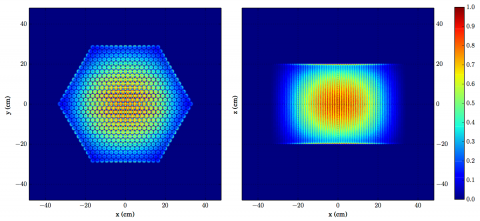
\includegraphics[height=1.5in,clip]{FissionSourceDistribution}
    \end{figure}

\end{frame}


%%%%%%%%%%%%%%%%%%%%%%%%%%%%%%%%%%%%%%%%%%%%%%%%%%%%%%
%%%%%%%%%%%%%%%%%%%%%%%%%%%%%%%%%%%%%%%%%%%%%%%%%%%%%%
\begin{frame}{Historical Context}
\begin{itemize}
\item Computing limitations of the past caused
\begin{itemize}
\item Heavy reliance on expensive and often complicated experiments
\item Inaccuracy resulted in \emph{significant design margins} $\rightarrow$ negative impact on plant economics
\item Exploration of novel reactor design concepts was greatly constrained by fundamental limitations in the predictability of the models
\vspace*{1 em}
\end{itemize}
\item Many codes (methods+implementation) developed then are still used 
\pause
\item Can we update these tools or do we need new ones?
\pause
\item What \textit{methods} will take us into the future?
\pause
\item What will the architectures look like?
\pause
\item What and how do we need to include other physics?
\end{itemize}
\end{frame}


%%%%%%%%%%%%%%%%%%%%%%%%%%%%%%%%%%%%%%%%%%%%%%%%%%%%%%
%%%%%%%%%%%%%%%%%%%%%%%%%%%%%%%%%%%%%%%%%%%%%%%%%%%%%%
\begin{frame}{This Class}

We will focus on
\begin{itemize}
\item Understanding the mathematical model (more of that in 250)
\item Learning computational methods (most of class)
\item (possibly) A little bit of implementation (take a computing class for this)
\item Assessing the answer
\end{itemize}
\end{frame}


%%%%%%%%%%%%%%%%%%%%%%%%%%%%%%%%%%%%%%%%%%%%%%%%%%%%%%
%%%%%%%%%%%%%%%%%%%%%%%%%%%%%%%%%%%%%%%%%%%%%%%%%%%%%%
\begin{frame}{Supercomputing in Research}
These kinds of simulations require time on the fastest computers in the world
\begin{itemize}
\item \textcolor{RawSienna}{Titan} (ORNL): 299,008 Opteron Cores (CPU) + 18,688 K21 Keplers (GPU); \textcolor{dgreen}{27 petaflops}
\item \textcolor{RawSienna}{IBM Sequoia} (LLNL): 1,572,864 cores (CPU); \\\textcolor{dgreen}{16.32 petaflops}
\end{itemize}
\begin{figure}
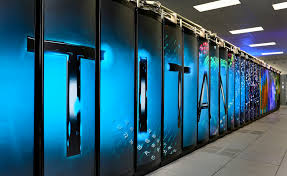
\includegraphics[height=1.1in,clip]{Titan}
\hfill
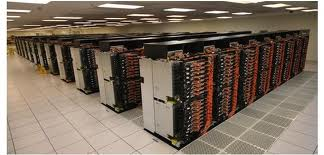
\includegraphics[height=1.1in,clip]{Sequoia}
\end{figure}
\end{frame}


%%%%%%%%%%%%%%%%%%%%%%%%%%%%%%%%%%%%%%%%%%%%%%%%%%%%%%
%%%%%%%%%%%%%%%%%%%%%%%%%%%%%%%%%%%%%%%%%%%%%%%%%%%%%%
\begin{frame}{What Can We Accomplish?}
\begin{itemize}
\item Predictive simulation 
\item Model entire facilities at a new level of fidelity
\item Coupled multi-physics
%Lets us reduce margins, extend existing reactor lifetimes, and consider new designs.
\end{itemize}
\begin{figure}
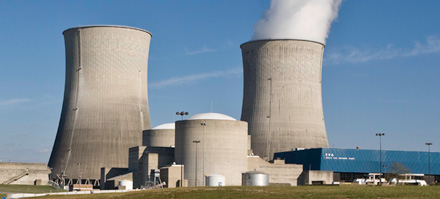
\includegraphics[height=1.2in,clip]{WattsBar}
\hfill
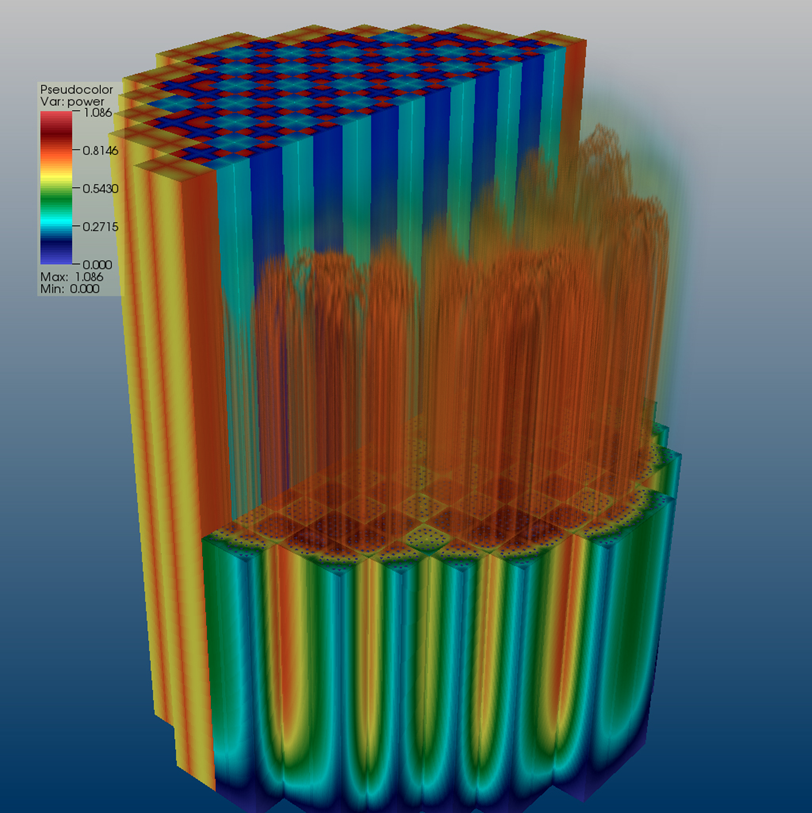
\includegraphics[height=1.2in,clip]{DenovoCore}
\end{figure}
\end{frame}


%%%%%%%%%%%%%%%%%%%%%%%%%%%%%%%%%%%%%%%%%%%%%%%%%%%%%%
%%%%%%%%%%%%%%%%%%%%%%%%%%%%%%%%%%%%%%%%%%%%%%%%%%%%%%
\begin{frame}{What Can We Accomplish?}
\underline{Integrate}
\begin{itemize}
\item existing nuclear energy and nuclear national security modeling and simulation capabilities
\item and associated expertise
\item with high-performance computing
\end{itemize}    
to solve problems that were \emph{previously unthinkable or impractical} in terms of the computing power required to address them.

\vspace*{1em}
However, these computer simulations will not completely eliminate the need for \emph{experimental or measurement data} to confirm or ``validate" the software. 

\vspace*{1em}
\hspace*{0.25 in} John Wagner, INL
\end{frame}

%"Traditionally, reactor models for radiation dose assessments have considered just the reactor core, or a small part of the core," Wagner says. "However, we're now simulating entire nuclear facilities, such as a nuclear power reactor facility with its auxiliary buildings and the ITER fusion reactor, with much greater accuracy than any other organization that we're aware of." 
%
%More accurate models enable nuclear plants to be designed with more accurate safety margins and shielding requirements, which helps to improve safety and reduce costs. The technology that makes this sort of leading-edge simulation possible is a combination of ORNL's Jaguar, the world's fastest supercomputer; advanced transport methods; and a next-generation software package called Denovo.
%
%DENOVO is a Scalable HPC Transport Code for Multi-Scale Nuclear Energy Applications
%http://computing.ornl.gov/SC09/videos/tomevans_1Mb.mov


%%%%%%%%%%%%%%%%%%%%%%%%%%%%%%%%%%%%%%%%%%%%%%%%%%%%%%
%%%%%%%%%%%%%%%%%%%%%%%%%%%%%%%%%%%%%%%%%%%%%%%%%%%%%%
\begin{frame}{Current State: CASL}
2010: the DOE announced \emph{Oak Ridge National Laboratory} won the Nuclear Energy Modeling and Simulation Energy Innovation Hub (awarded 5 more years in 2015), including:	
\begin{itemize}
\item Electric Power Research Institute (EPRI), Palo Alto, CA
\item Idaho National Laboratory, Idaho Falls, ID
\item Los Alamos National Laboratory, Los Alamos, NM
\item Massachusetts Institute of Technology, Cambridge, MA
\item North Carolina State University, Raleigh, NC
\item Sandia National Laboratories, Albuquerque, NM
\item Tennessee Valley Authority, Knoxville, TN
\item University of Michigan, Ann Arbor, MI
\item Westinghouse Electric Company, Pittsburgh, PA
\end{itemize}
\end{frame}

%%%%%%%%%%%%%%%%%%%%%%%%%%%%%%%%%%%%%%%%%%%%%%%%%%%%%%
%%%%%%%%%%%%%%%%%%%%%%%%%%%%%%%%%%%%%%%%%%%%%%%%%%%%%%
\begin{frame}{Consortium for Advanced Simulation of Light Water Reactors}
\begin{center}

\includegraphics[height=0.65in,clip]{CASL}
\end{center}
\begin{itemize}
\item CASL's focus is on \textit{currently operating light water reactors}.
\item They've developed the Virtual Environment for Reactor Applications, \textbf{VERA}, which simulates nuclear reactor physical phenomena using coupled multi-physics models.
\item They have LWR-specific challenge problems such as GTRF, CRUD, PCI, DNB, FAD, RPV internals, etc. \end{itemize}
\end{frame}


%%%%%%%%%%%%%%%%%%%%%%%%%%%%%%%%%%%%%%%%%%%%%%%%%%%%%%
%%%%%%%%%%%%%%%%%%%%%%%%%%%%%%%%%%%%%%%%%%%%%%%%%%%%%%
\begin{frame}{Current State: MOOSE and SHARP}

\begin{itemize}
\item \textcolor{RawSienna}{MOOSE}: The Multiphysics Object-Oriented Simulation Environment (MOOSE) is a finite-element, multiphysics framework primarily developed by Idaho National Lab. It provides a high-level interface to some of the most sophisticated nonlinear solver technology on the planet.
\pause
\vspace*{1 em}
\item \textcolor{RawSienna}{SHARP}: The Simulation-based High-efficiency Advanced Reactor Prototyping (SHARP) suite of codes enables virtual design and engineering of nuclear plant behavior...researchers (Argonne National Lab) have developed a set of simulation tools that provide a highly detailed description of the reactor core and the nuclear plant behavior. 
\end{itemize}
\end{frame}


%%%%%%%%%%%%%%%%%%%%%%%%%%%%%%%%%%%%%%%%%%%%%%%%%%%%%%
%%%%%%%%%%%%%%%%%%%%%%%%%%%%%%%%%%%%%%%%%%%%%%%%%%%%%%
\begin{frame}{Quick Comparison}
\begin{center}
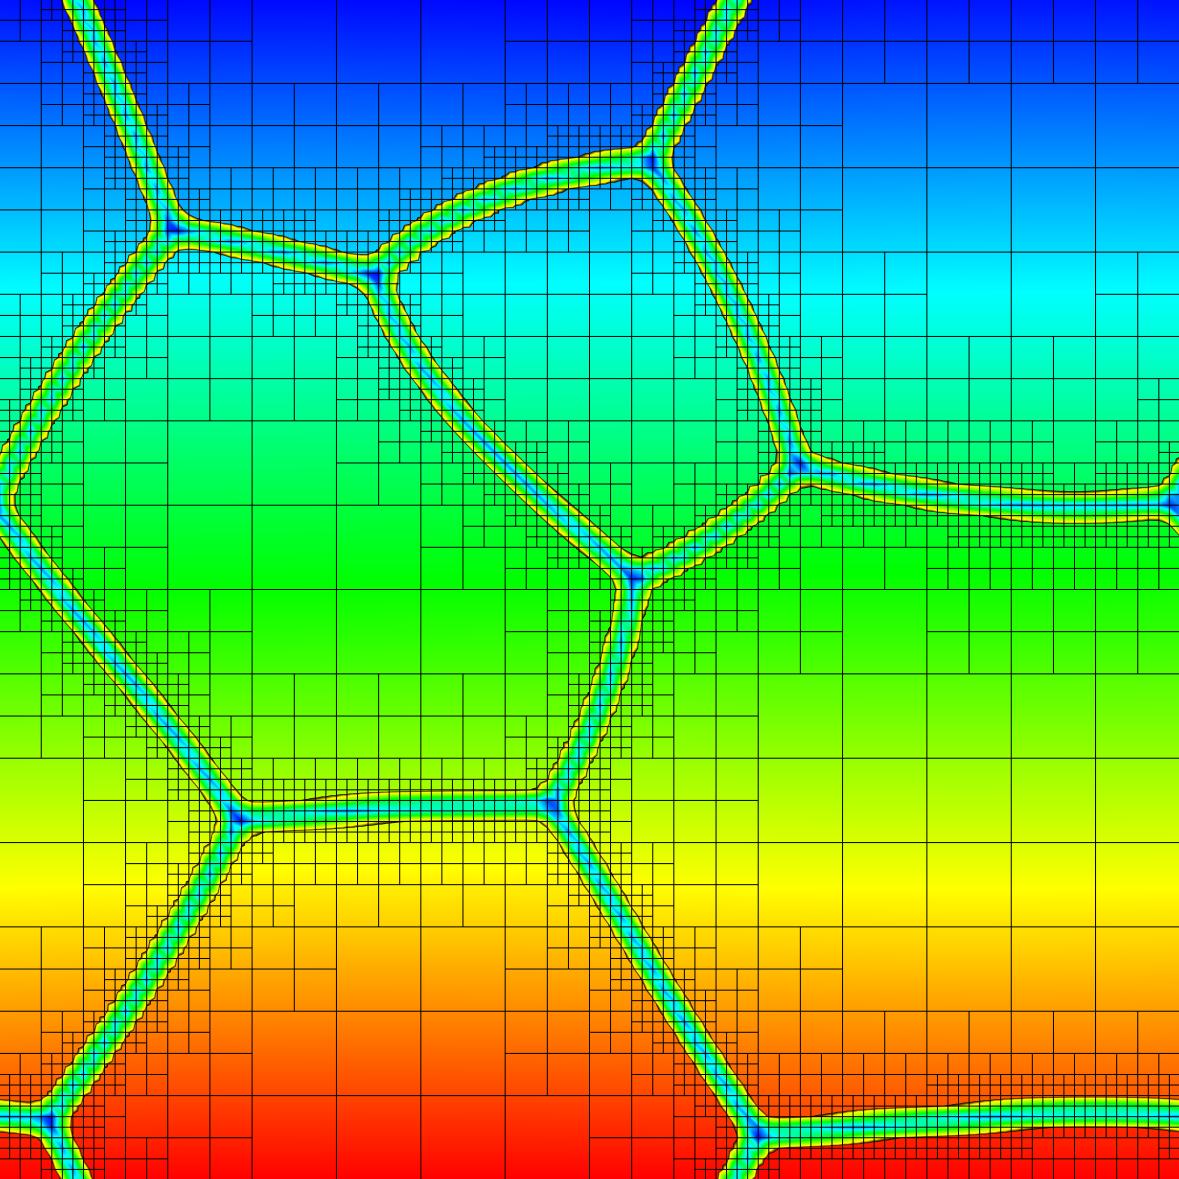
\includegraphics[height=0.75in,clip]{moose}
\end{center}
\begin{itemize}
\item MOOSE and SHARP focus more heavily on advanced reactor design.
\item They have package that address more types of physics than CASL.
\item MOOSE is open source, though many of the ``animals" that do the physics are not.
\item MOOSE and SHARP are supported by DOE Office of Nuclear Energy, while CASL is the Office of Science.
\end{itemize}
\end{frame}


%%%%%%%%%%%%%%%%%%%%%%%%%%%%%%%%%%%%%%%%%%%%%%%%%%%%%%
%%%%%%%%%%%%%%%%%%%%%%%%%%%%%%%%%%%%%%%%%%%%%%%%%%%%%%
\begin{frame}{What Are People Working on Now?}
Examples from DOE-NE funding opportunity announcement
\begin{itemize}
\item Advanced Reactor Methods Topics
  \begin{itemize}
  \item Sodium Fast Reactor
  \item High Temperature Gas Reactor
  \item Molten Salt Reactor
  \end{itemize}
\item Reactor Concepts
\item Nuclear Energy Advanced Modeling and Simulation (NEAMS): Core Neutronics
\item Grand Challenge Problem for Nuclear Energy
\item Critical Data Needs for NEAMS
\end{itemize}

\end{frame}


%%%%%%%%%%%%%%%%%%%%%%%%%%%%%%%%%%%%%%%%%%%%%%%%%%%%%%
%%%%%%%%%%%%%%%%%%%%%%%%%%%%%%%%%%%%%%%%%%%%%%%%%%%%%%
\begin{frame}{Are You Up To the Challenge?}
\begin{figure}

\includegraphics[height=2.5in,clip]{science}
\end{figure}
\end{frame}

\end{document}
